\documentclass[preprint]{article}

% if you need to pass options to natbib, use, e.g.:
%     \PassOptionsToPackage{numbers, compress}{natbib}
% before loading neurips_2023

% ready for submission
\usepackage{neurips_2023}


% to compile a preprint version, e.g., for submission to arXiv, add add the
% [preprint] option:
%     \usepackage[preprint]{neurips_2023}


% to compile a camera-ready version, add the [final] option, e.g.:
%     \usepackage[final]{neurips_2023}


% to avoid loading the natbib package, add option nonatbib:
%    \usepackage[nonatbib]{neurips_2023}


\usepackage[utf8]{inputenc} % allow utf-8 input
\usepackage[T1]{fontenc}    % use 8-bit T1 fonts
\usepackage{hyperref}       % hyperlinks
\usepackage{url}            % simple URL typesetting
\usepackage{booktabs}       % professional-quality tables
\usepackage{amsfonts}       % blackboard math symbols
\usepackage{nicefrac}       % compact symbols for 1/2, etc.
\usepackage{microtype}      % microtypography
\usepackage{xcolor}         % colors
\usepackage{listings}
\usepackage{cite}
\usepackage{graphicx}
\usepackage{hyperref}
\usepackage{array}



\lstset{
  breaklines=true,
  basicstyle=\ttfamily\small,
  commentstyle=\color{green!40!black},
  keywordstyle=\color{blue},
  numberstyle=\tiny\color{gray},
  numbers=none,
  frame=single,
  breaklines=true,
  breakatwhitespace=true,
  captionpos=b,
  showstringspaces=false,
  columns=fullflexible,
}

\hypersetup{
    pdftitle={MMMModal - Multi-Images Multi-Audio Multi-turn Multi-Modal},
    pdfauthor={Husein Zolkepli, Aisyah Razak,  Kamarul Adha, Ariff Nazhan},
    pdfsubject={Natural Language Processing, Large Language Models, Machine Learning},
    pdfkeywords={language models, natural language processing, deep learning},
    colorlinks=true,
    linkcolor=blue,
    citecolor=blue,
    urlcolor=blue
}
\title{MMMModal - Multi-Images Multi-Audio Multi-turn Multi-Modal}
\author{
  Husein Zolkepli\thanks{husein@mesolitica.com} \and
  Aisyah Razak\thanks{aisyahrazak171@gmail.com} \and
  Kamarul Adha\thanks{kamarul.adha360@gmail.com} \and
  Ariff Nazhan\thanks{ariffnzhn@gmail.com}
}

\begin{document}

\maketitle

\begin{abstract}

  Our contribution introduces a groundbreaking multimodal large language model designed to comprehend multi-images, multi-audio, and multi-images-multi-audio within a single multiturn session. Leveraging state-of-the-art models, we utilize the SigLIP encoder for visual inputs and the Whisper Encoder for audio inputs. Notably, this multimodal large language model is bilingual, proficient in understanding both English and Malay simultaneously. We proudly unveil three versions of this model: Qwen1.5 with 0.5B parameters, TinyLlama with 1.1B parameters, and Mistral with 7B parameters. With its ability to navigate diverse modalities and languages, our model represents a significant advancement for the Malaysian context and beyond.

  All models released at \href{https://huggingface.co/collections/mesolitica/multimodal-malaysian-llm-65c6f893e03f78fa9e5c8859}{HuggingFace Mesolitica Multimodal Malaysian LLM}.

\end{abstract}

\section{Introduction}

Language models trained with instructions have shown remarkable performance across various domains. However, their limitation in handling only text-based data hampers their applicability. Recent advancements in multimodal pre-training have demonstrated the potential to integrate knowledge from diverse modalities into a unified representation.\cite{lyu2023macawllm}\cite{liu2023visual} Despite these advancements, there remains a lack of existing multimodal models capable of supporting multiple images/audio inputs and multiturn dialogue in current research. Addressing this gap, our proposal introduces MMModal, a multi-modal instruction-tuned Language Learning Model (LLM) that combines image, audio, and text modalities within a single model architecture.

\begin{itemize}

  \item \textbf{Synthetic Audio Instruction Dataset:} In the realm of Natural Language Processing (NLP), research indicates that the quality of instruction-following data significantly impacts the efficacy of instruction-following models. To illustrate this, we create a synthetic dataset comprising multi-dialogue interactions involving multiple images and audio inputs. Using Mistral, we generate a multiturn dialogue instruction dataset aimed at enhancing the language model's capacity to produce precise and contextually relevant responses. This dataset encompasses three distinct types of instruction-following data: multiple images instructions,
        multi-audio instructions, and combined image and audio instructions.

  \item \textbf{Synthetic Visual Malaysian Context Dataset:} a

  \item \textbf{Synthetic Multi-Images Multi-Audio relationship Dataset:} Our approach adopts a two-step training procedure to integrate multimodal and multiturn capabilities into our model. The initial step entails pretraining the feature alignment module. Through this process, we align the image features and audio data with the pre-trained word embeddings of the Language Learning Model (LLM). Specifically, this step involves training the projection layer to ensure alignment between the multi-modal features and textual representations. This alignment facilitates seamless integration of diverse modalities within the model architecture.

  \item \textbf{Pretraining Feature Alignment:} a

  \item \textbf{Finetuned Multi-Images Multi-Audio Multi-turn Model:} a

\end{itemize}

\section{Synthetic Data Generation for Audio Instructions}

\section{Synthetic Visual Malaysian Context Dataset}

\section{Synthetic Data Generation for Multi-Images, Multi-Audio Multi-turn Instructions}

\subsection{Synthetic Multi-Images Instruction}

\subsection{Synthetic Multi-Audio Instruction}

\subsection{Synthetic Image-Audio Instruction}

\section{Finetuning Procedure}

\subsection{Overall Architecture}

\subsection{Pretraining for Visual Feature Alignment}

\subsection{Pretraining for Audio Feature Alignment}

\subsection{Instruction Finetuning}

The fine-tuning hyperparameters are detailed below:

\begin{table}[h]
  \centering
  \begin{tabular}{lccl}
    \hline
    \textbf{Hyperparameter} & \textbf{Value} \\
    \hline
    DeepSpeed               & ZeRO-2 Offload \\
    Batch Size              & 12             \\
    Learning Rate           & constant 2e-5  \\
    Precision               & bfloat16       \\
    \hline
  \end{tabular}
\end{table}

Complete fine-tuning 8192 context length implementation at \href{https://github.com/mesolitica/multimodal-LLM/blob/master/run-deepspeed.sh}{here}.

\section{Examples}

This section presents examples that highlight the model's capacity to comprehend and produce responses relating to visual and audio input, showcasing the efficacy and potential of our proposed MMModal. These examples clearly demonstrate how the model handles and combines various information modalities, including audio and pictures, in the context of natural language processing (NLP). MMModal exhibits its capability by producing insightful, pertinent, and cohesive answers to a diverse set of inquiries. This highlights the model's capacity to create exceptionally efficient interfaces for human-machine communication.

\begin{table}[hbt!]
  \setlength{\extrarowheight}{3pt} % Adjust the value as needed
  \renewcommand{\arraystretch}{1.5} % Adjust the value as needed
  \begin{tabular}{lcccl}
    \hline
    \textbf{Multi Images Input Example}                                                                                                                    \\[6pt]  % Adjust the value as needed
    \hline
    \hline
    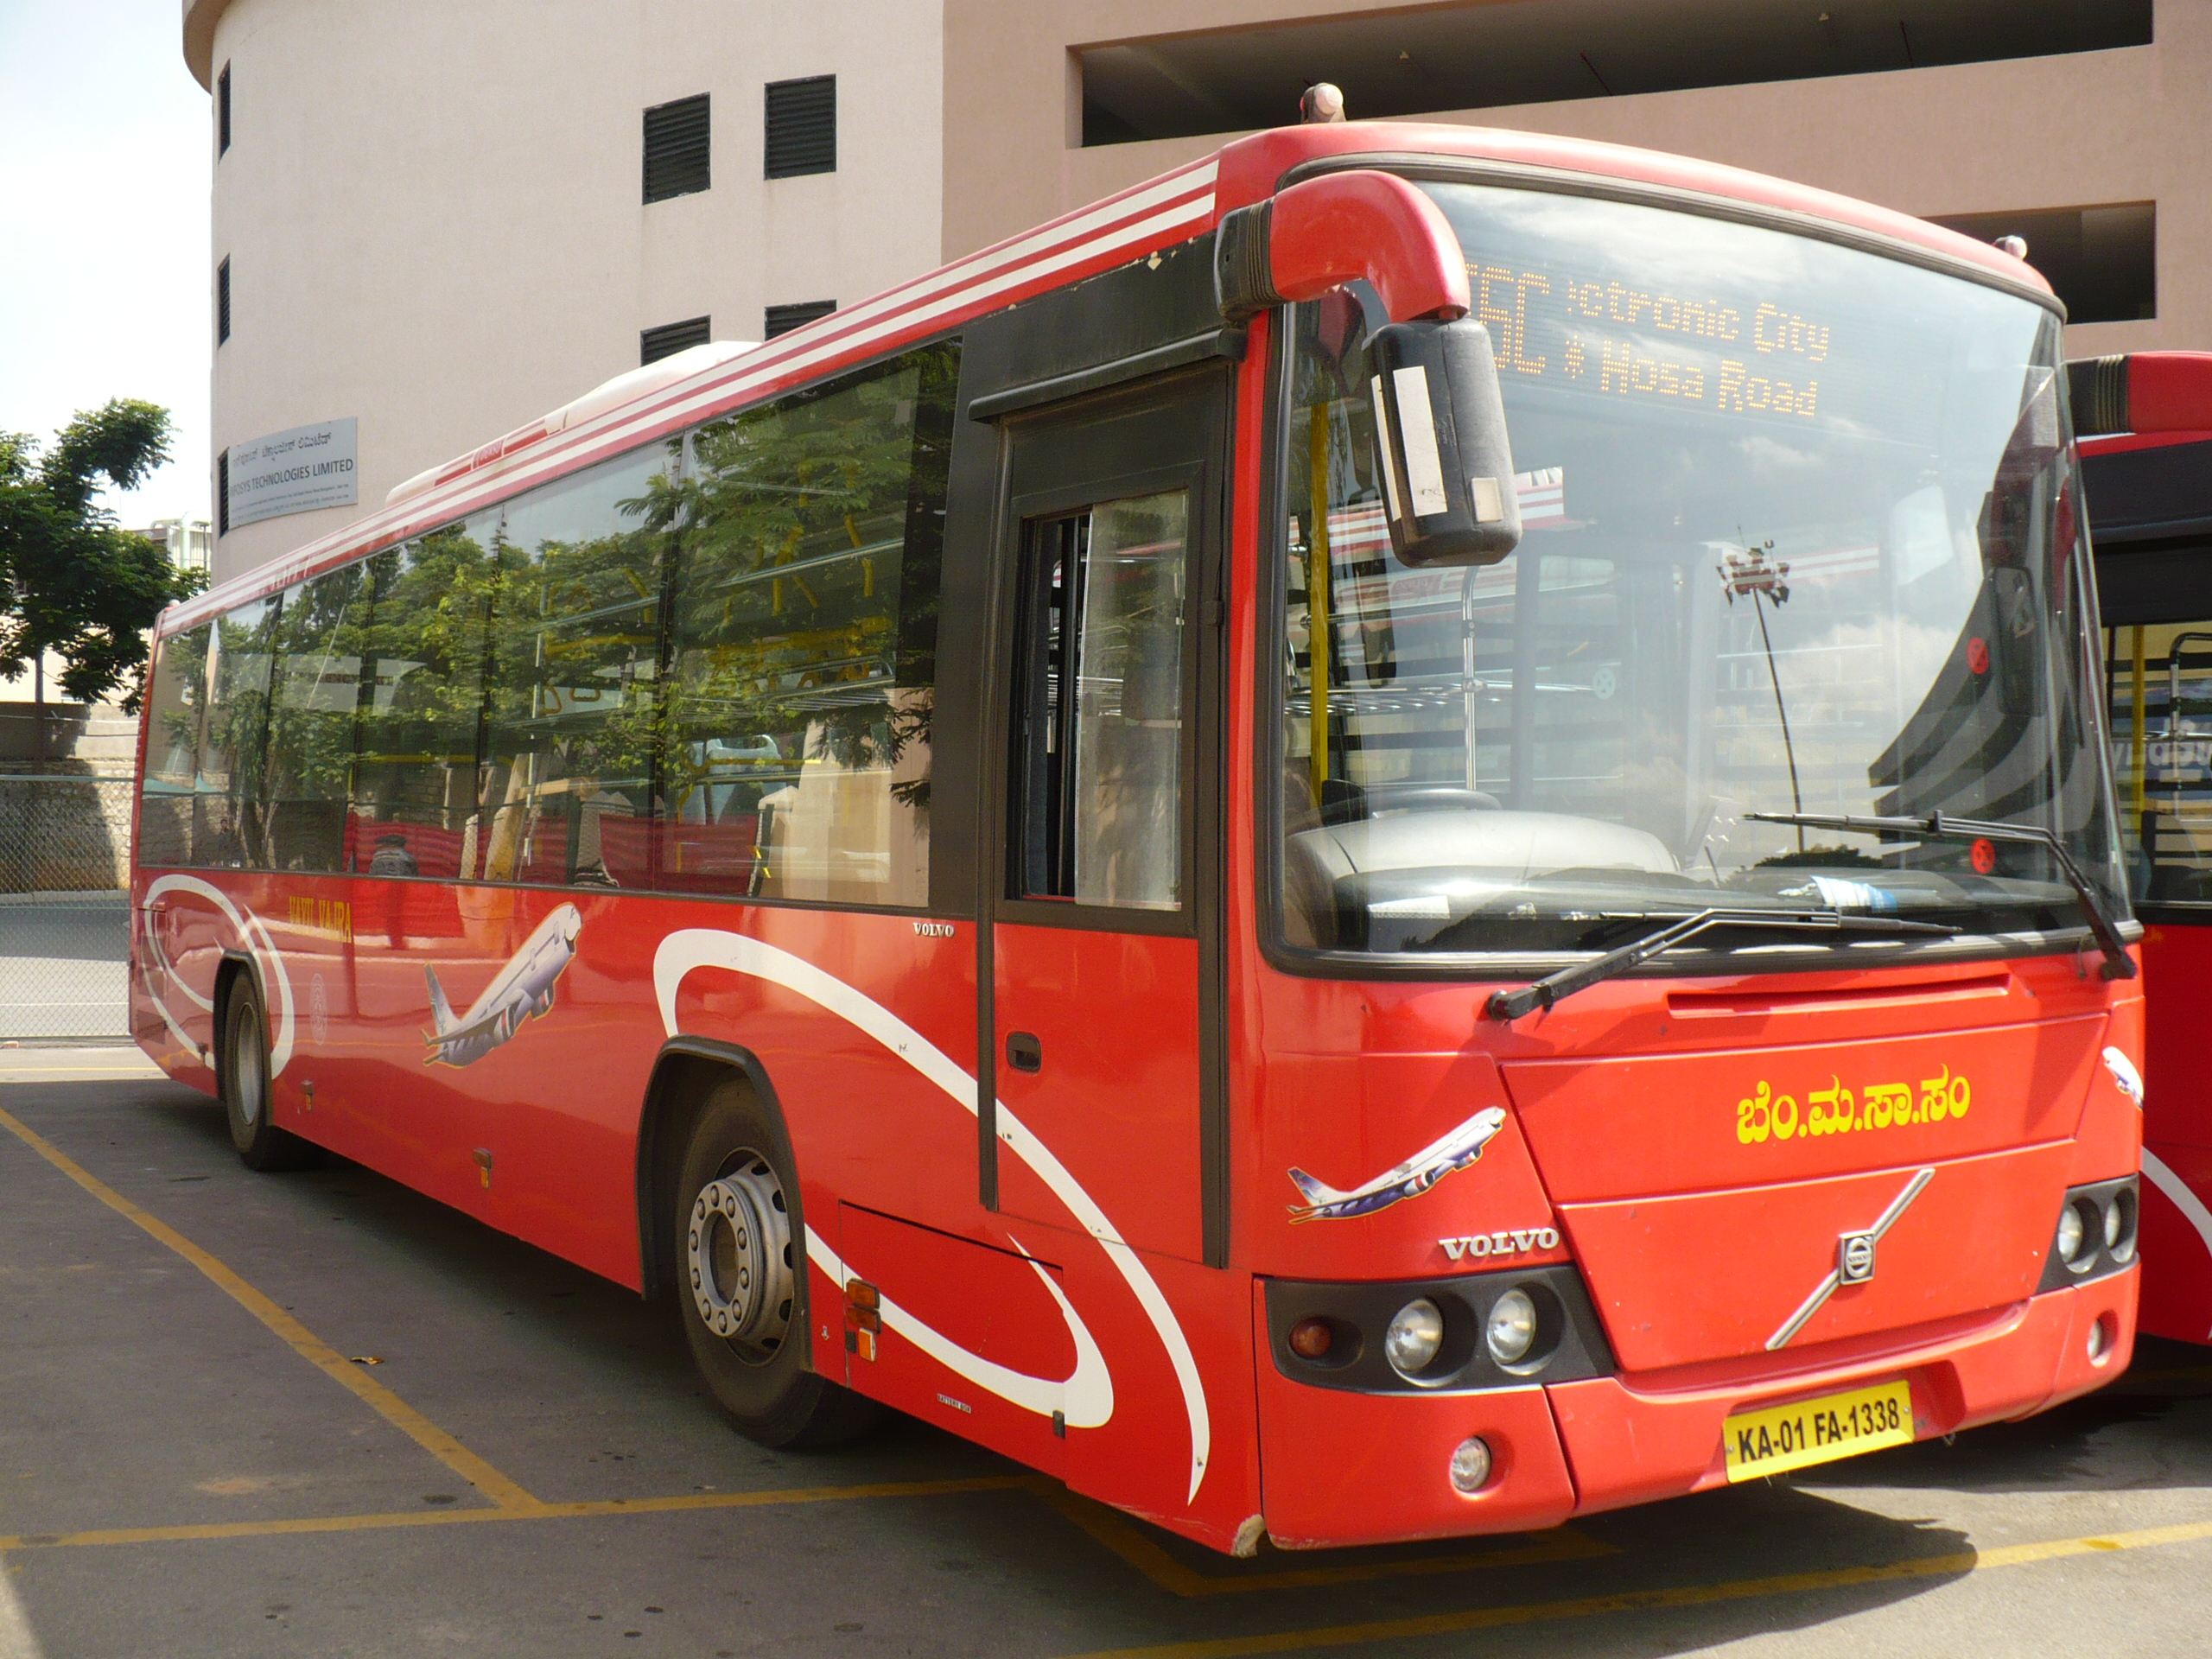
\includegraphics[width=0.45\linewidth,keepaspectratio]{pic/R.jpeg} & 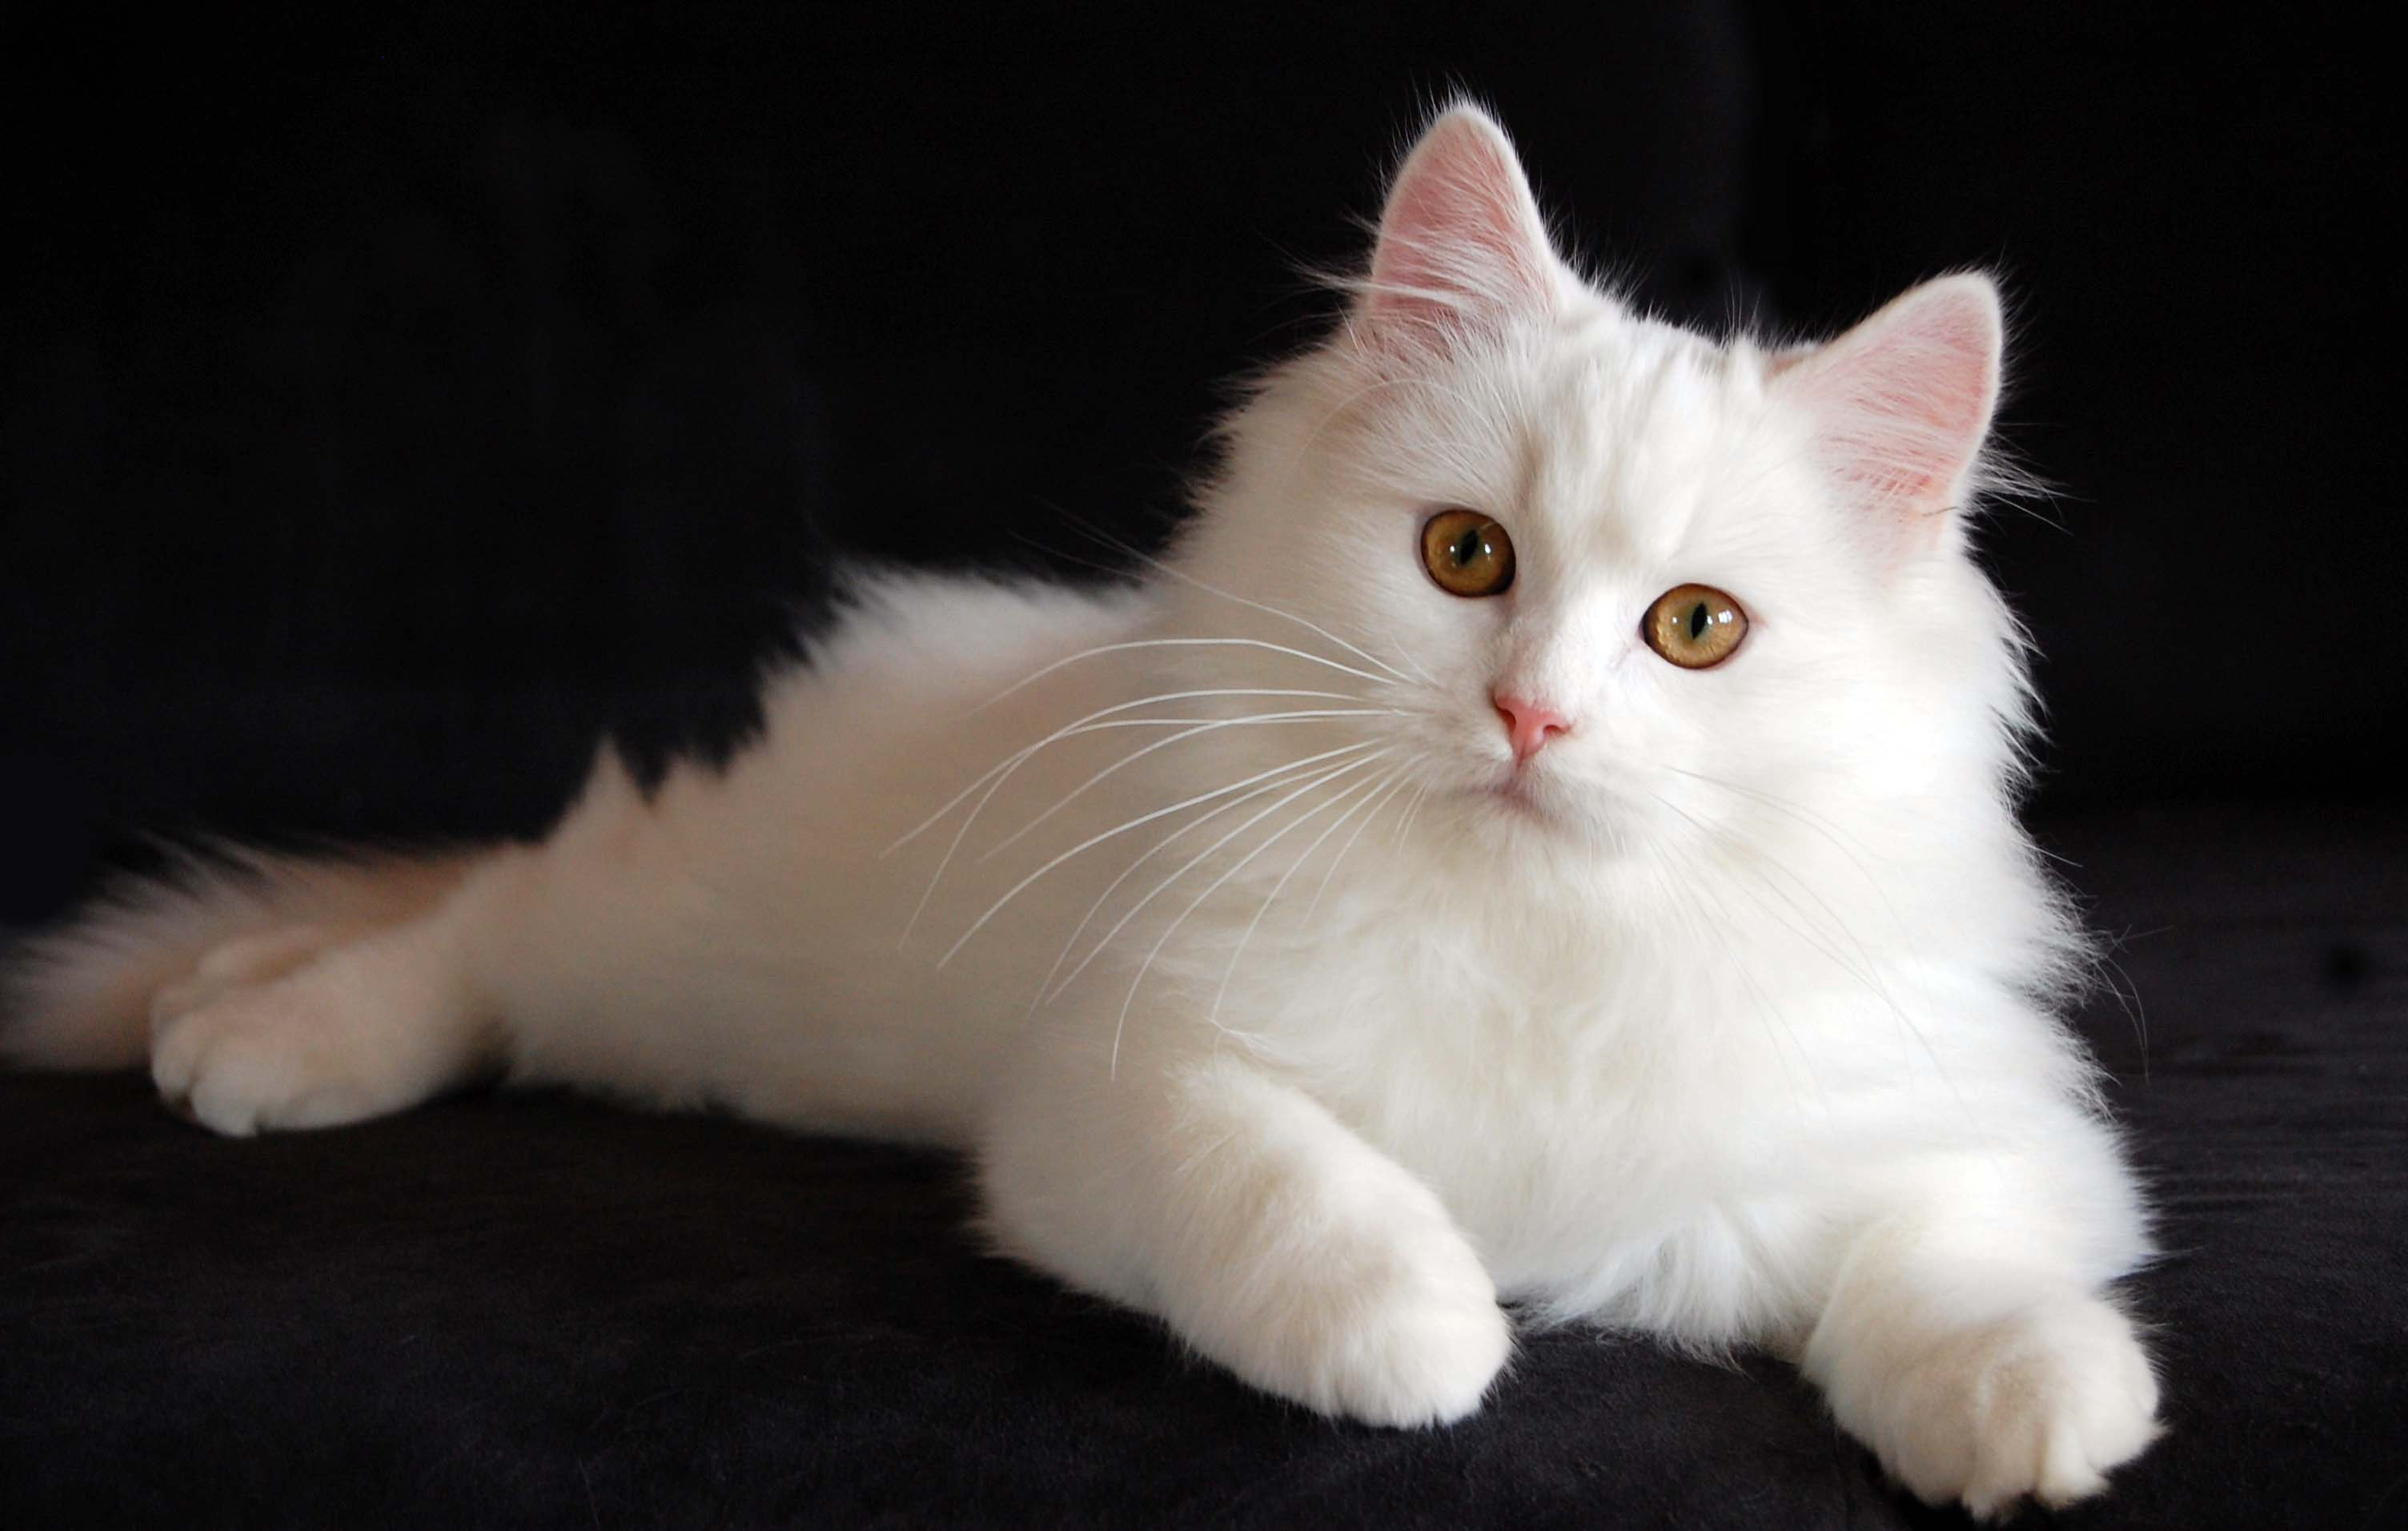
\includegraphics[width=0.45\linewidth,keepaspectratio]{pic/Persian-cat-breed.jpg} \\
    User                                                               & What is related between image 1 and image 2?                                      \\
    \hline
  \end{tabular}
\end{table}

\begin{table}[hbt!]
  \setlength{\extrarowheight}{3pt} % Adjust the value as needed
  \renewcommand{\arraystretch}{1.5} % Adjust the value as needed
  \begin{tabular}{lcccl}
    \hline
    \textbf{Multi Audio Input Example}                                                                                                                     \\[6pt]  % Adjust the value as needed
    \hline
    \hline
    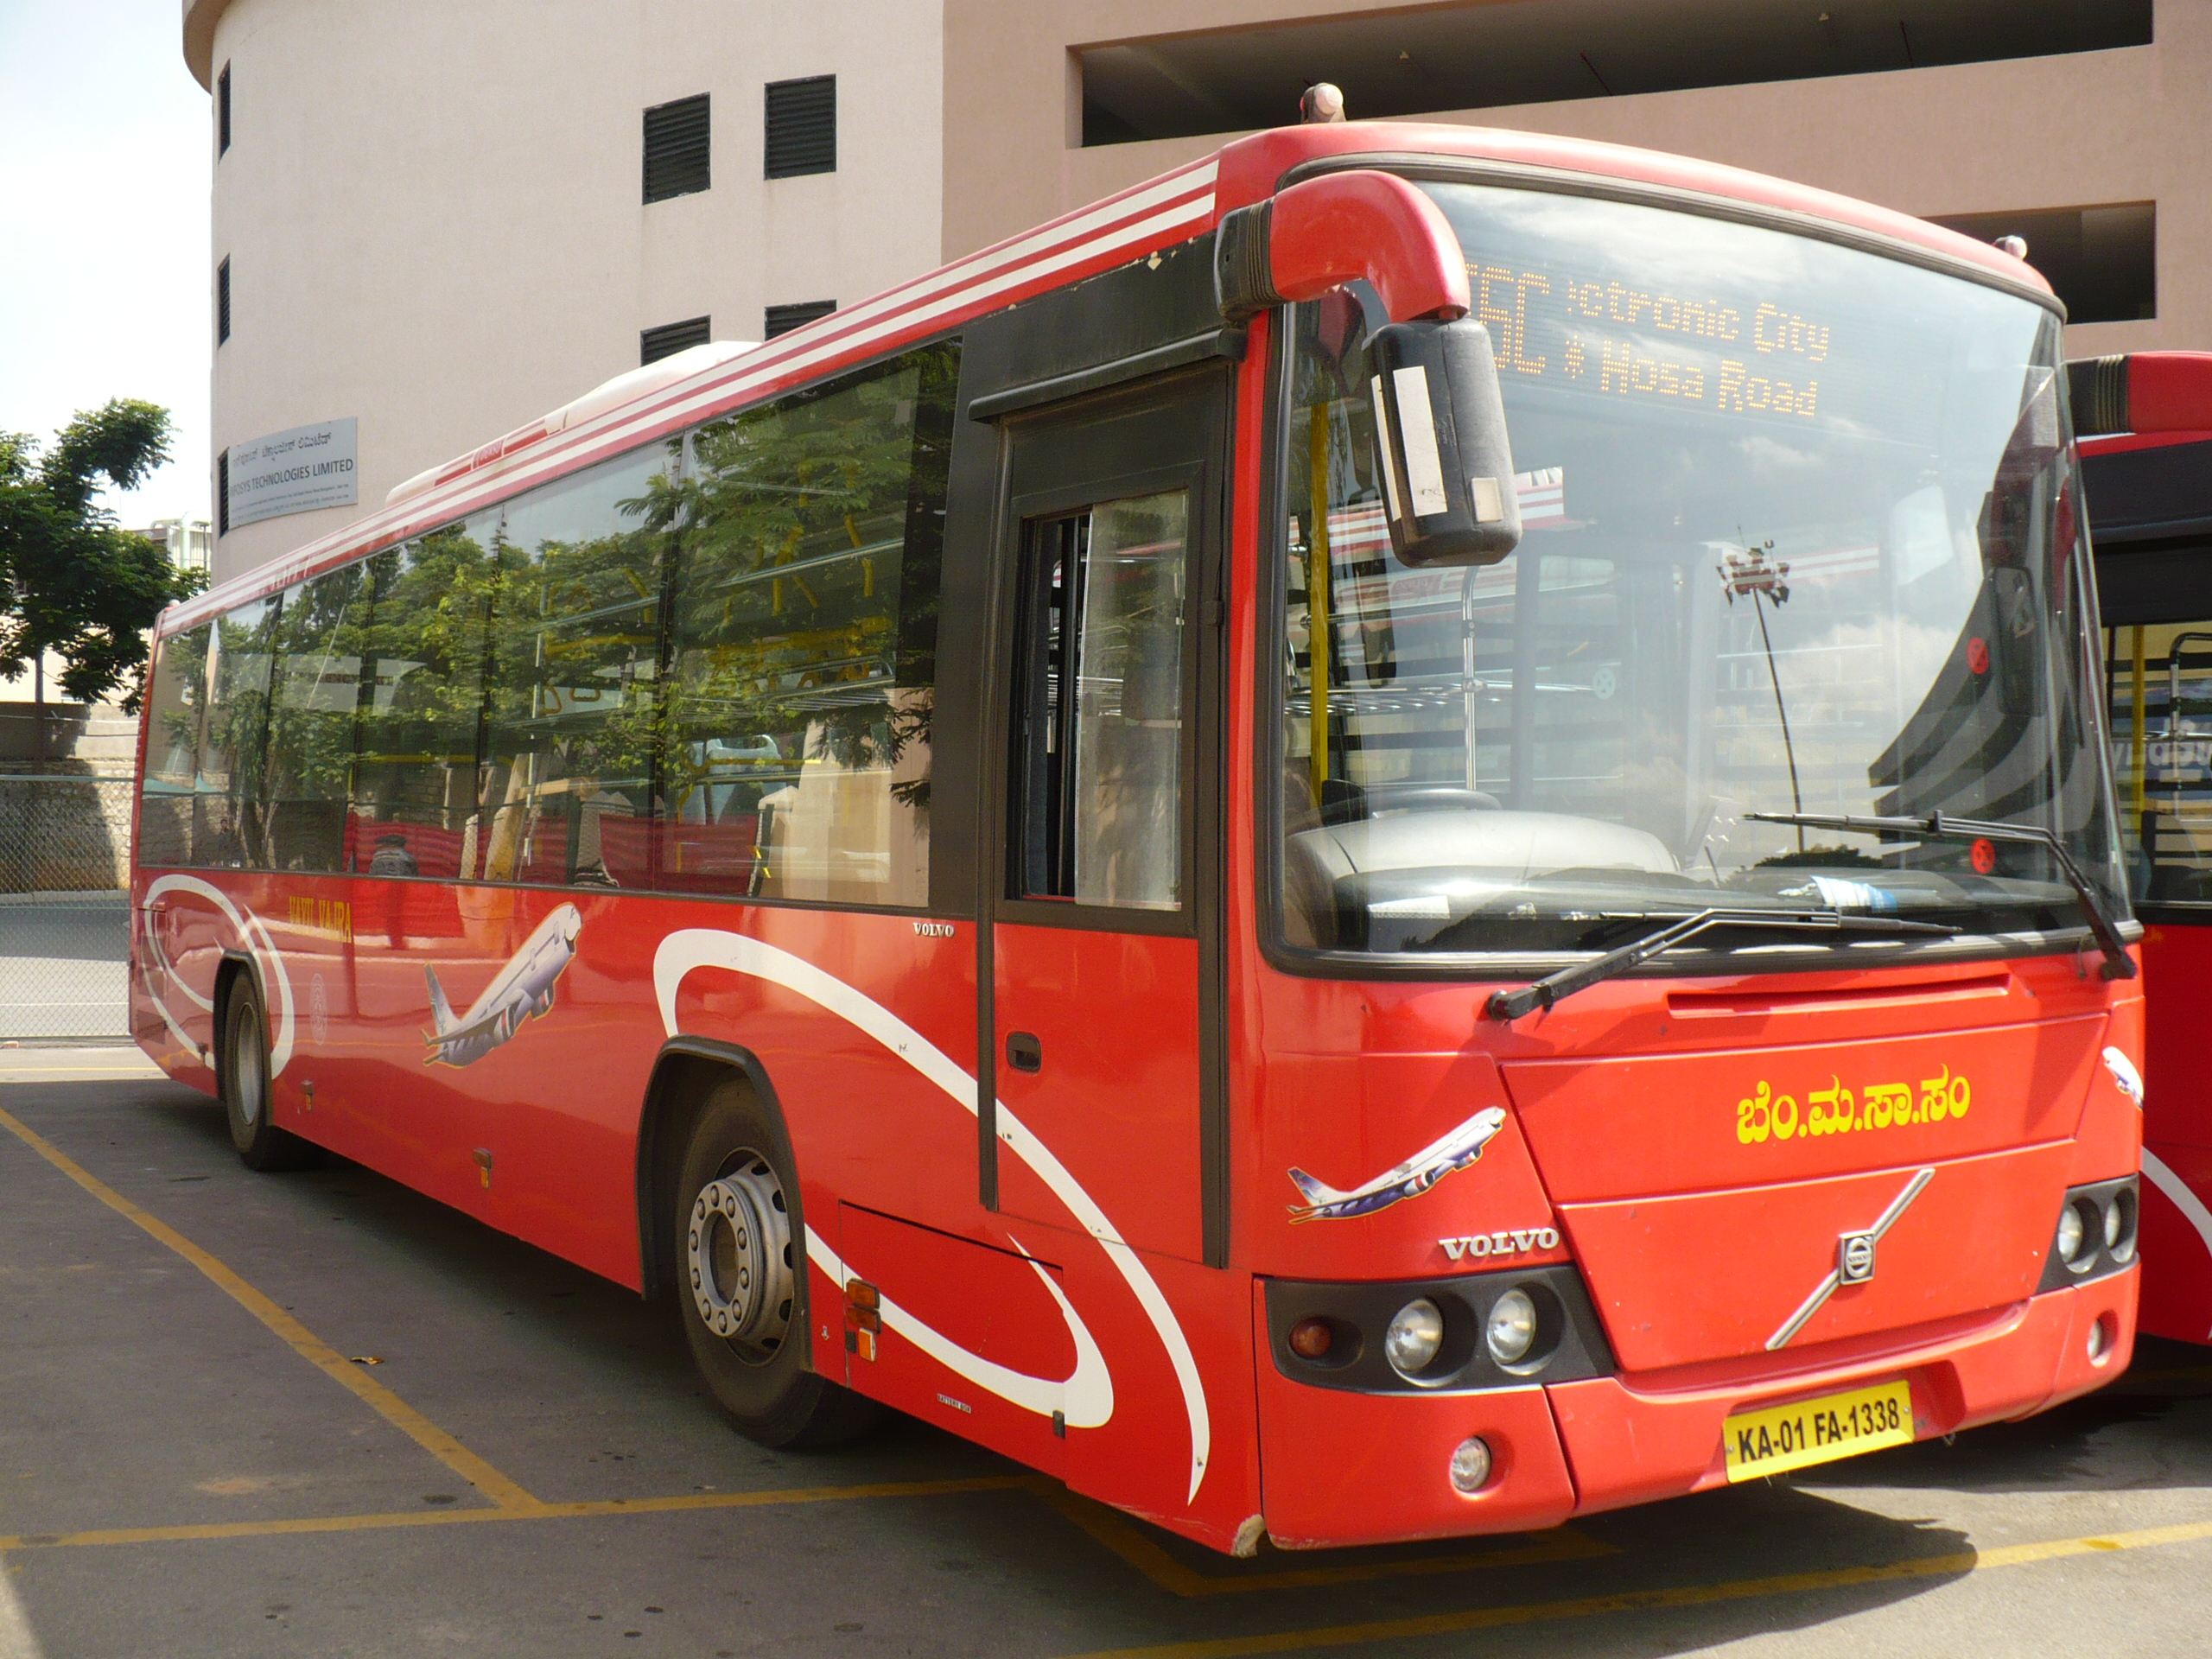
\includegraphics[width=0.45\linewidth,keepaspectratio]{pic/R.jpeg} & 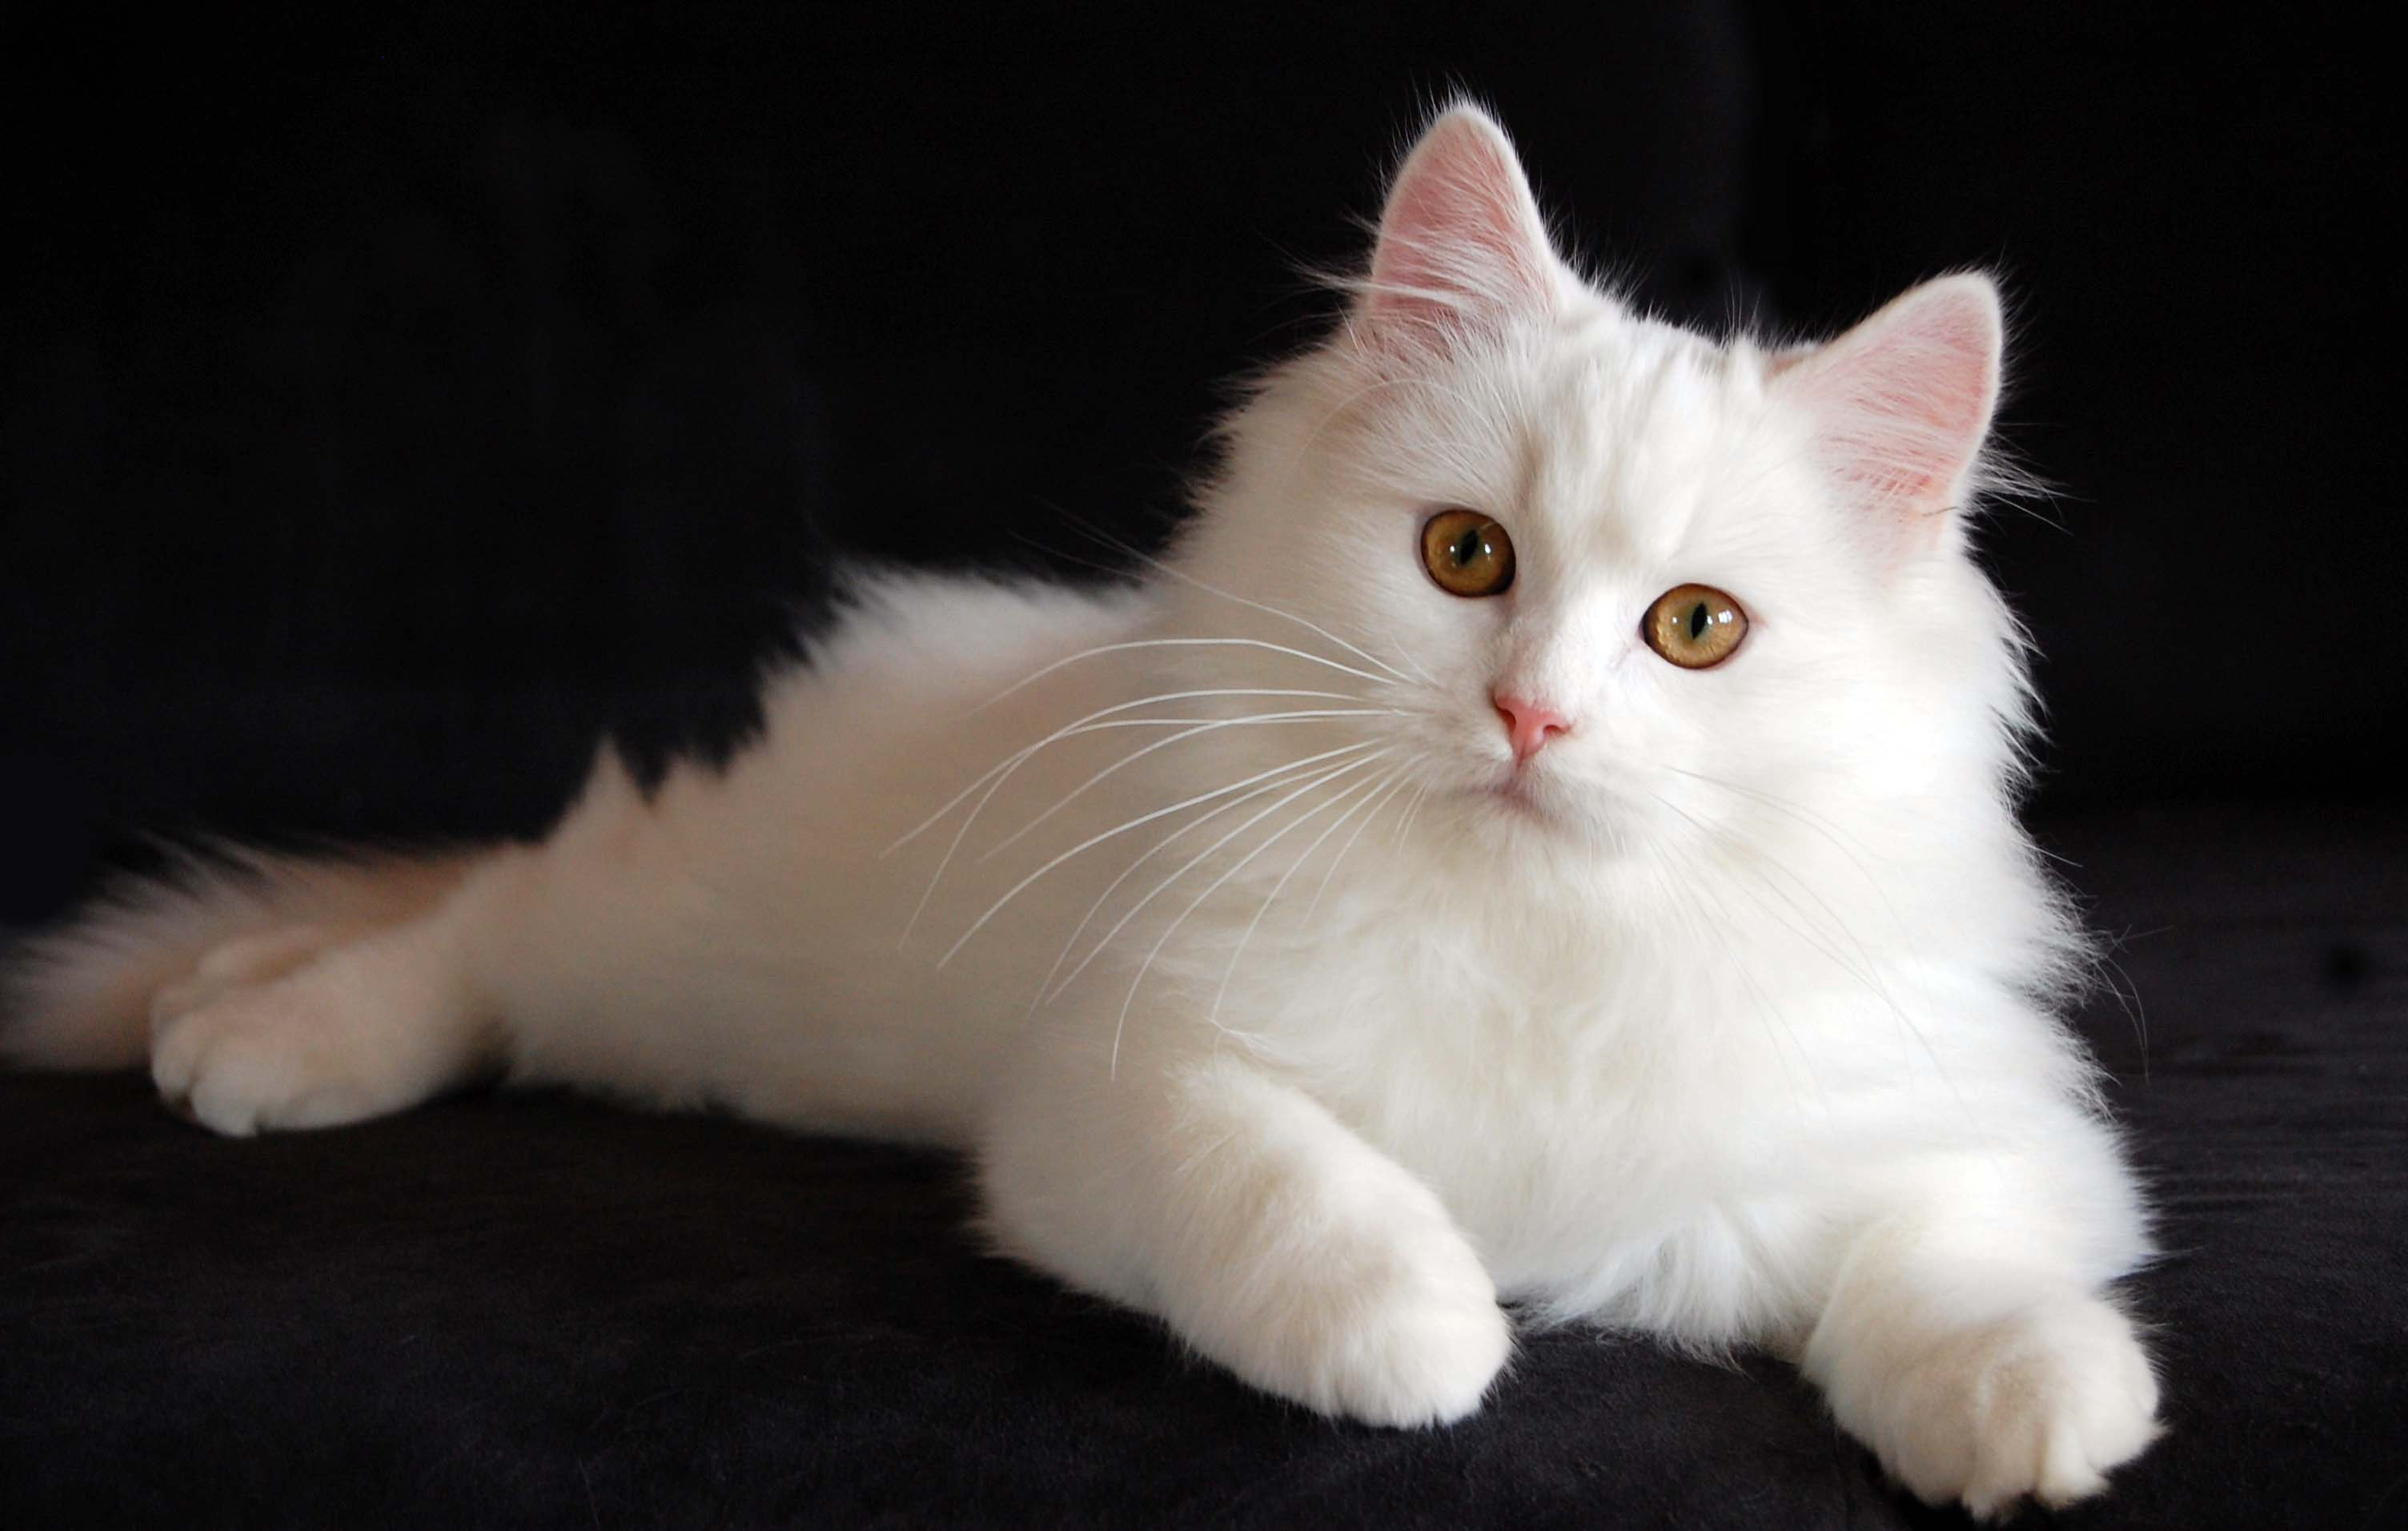
\includegraphics[width=0.45\linewidth,keepaspectratio]{pic/Persian-cat-breed.jpg} \\
    User                                                               & What is related between audio 1 and audio 2?                                      \\
    \hline
  \end{tabular}
\end{table}


\section{Evaluation}

\section{Future Work}

In our future endeavors, we aim to enhance our capabilities by focusing on several key areas. Firstly, we intend to refine our approach to generating synthetic datasets that incorporate multi-images and multi-audio inputs. This will involve expanding the dataset to include more complex relationships between inputs and facilitating comparisons involving more than two inputs. Additionally, we recognize the importance of incorporating a wider range of visual Malaysian context datasets into our model training pipeline. By diversifying our data sources, we can ensure that our model is equipped to handle a broader array of real-world scenarios and contexts, ultimately improving its performance and relevance in practical applications.

\section{Acknowledgement}

Special thanks to Malaysia-AI volunteers especially \href{https://www.linkedin.com/in/wan-adzhar-faiq-adzlan-19a27baa/}{Wan Adzhar Faiq Adzlan}, \href{https://www.linkedin.com/in/ammar-azman/}{Ammar Azman}, \href{https://www.linkedin.com/in/amzar96/}{M. Amzar}, \href{https://www.linkedin.com/in/muhammad-farhan-helmy-0529501a7/}{Muhammad Farhan}, \href{https://www.linkedin.com/in/syafie-nizam/}{Syafie Nizam}, \href{https://www.linkedin.com/in/halimshukor/}{Halim Shukor}, \href{https://www.linkedin.com/in/alif-aiman-1b334b24b/}{Alif Aiman}, \href{https://www.linkedin.com/in/azwan-zuharimi/}{Azwan Zuharimi} and \href{https://www.linkedin.com/in/haziqzikry/}{Haziq Zikry} for contributing dataset to train MMMModal.

We would like to express our gratitude to NVIDIA Inception for generously providing us with the opportunity to train our model on the Azure cloud. Their support has played a crucial role in the success of our research, enabling us to leverage advanced technologies and computational resources.

We extend our thanks to the wider research community for their valuable insights and collaborative discussions, which have greatly influenced our work. This paper reflects the collective efforts and contributions from both NVIDIA Inception and the broader research community.

\section{Conclusion}

In this paper, we introduce MMMModal, a multimodal instruction tuned Model (LLM) specifically designed to handle multiple modalities, including images, audio, and text in a multi-turn dialogue setting. Our novel approach focuses on aligning representations from various modality encoders into a unified space. Unlike existing methods, our approach enables the model to effectively process multi-turn dialogues and incorporate multiple images or audio inputs in its responses. We provide examples demonstrating the multi-modal understanding capabilities of MMMModal.

\bibliography{neurips_2023}{}
\bibliographystyle{unsrt}

\end{document}